\documentclass[11pt,twoside,a4paper]{article}
\usepackage{amsmath}
\usepackage{mathtools}
\usepackage{graphicx}
\graphicspath{ {/home/alisa/uni-sven/proj/pics/} }

\begin{document}
\title{Development and programming of a micro processor}
\author{Alisa Dammer and Sven-Hendrik Haase}
\maketitle

\section{Introduction}
\subsection{General information: How does CPU work}
A central processing unit (CPU) is a heart of a computer. It presents arithmnetical logic, logic operations and input-output operations. Nowadays one computer can have more than one CPU, called multiprocessors. But in this project we have concentrated our attention on one single microprocessor.\\
In order to work properly and execute commands (perform certain operations), CPU needs to go through several stages:
\begin{enumerate}
	\item[1.] Fetch: read the program, that is stored in memory as instructions. (We implemented an Assambeler, that translates the program from "human" language to instructions. More about it in  section "CPU implementation"). To keep an eye on right order of instructions Program Counter (PC) keeps the address of the next executable instruction.
	\item[2.] Decode: Instruction is a representation of a assembly command in 0 and 1. During this stage every executable instruction is broken up into several parts. The amount and length of these pieces depend on the type of instruction (more details in the next section). 
	\item[3.] Execute: According to what kind of instruction has to be performed, different units of the CPU can be involved. For example: ALU and two registers, or CU and register etc. Normally modern CPUs have overflow flags, that are "activated", if the output is too big for restricted CPU (by "restricted" we mean, that all CPUs are by design implemented to deal with limited values).
	\item[4.] Writeback: During this stage the result of an instruction is "returned" to some memory part, so that it could be used later on.
\end{enumerate}

All these 4 steps repeat for every instruction until the "stop" instruction is reached (logical end of the program), which is normally refers to "no action" or "terminate". As was mentioned above in Fetch-stage, PC holds the address of the next executable instruction, incrementing each time the instruction is executed. Some of control instructions like "jump" change PC according to needs of the program, for example by implementing a cycle.\\
\subsection{Main components of a simple CPU}
Every CPU's design starts with Instruction Set Architecture (ISA) definition, that describes what particular prozessor is capable of: general specification (word length, instruction length), instruction specifications and opcodes (operations, that can be presented in binary form), type of memory that is used (number of special purpose and general purpose registers), and other specific infromation if needed. \\
Apart from ISA all microprozessors have certain units like: Program Counter (PC), Control Unit (CU), Aruthmetic Logic Unit (ALU), Registers (Register Bank), Buses.\\
\begin{center}
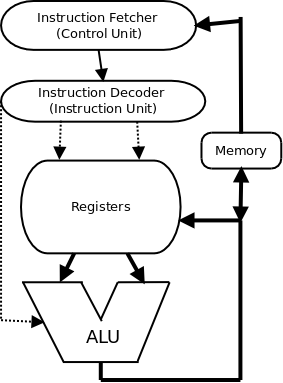
\includegraphics[scale=0.5]{simpleCPU3.png}
\end{center}

However our implementation differs from existing ones. This will be shown in details in next section.\\ 

\newpage
\section{CPU implementation}
\subsection{Instruction Set Architecture}
As was mentioned in the previous section, ISA defines all specifications of a CPU. In our work we decided to stop on 16bit instructions, that have the same lenght as word, so we didn't have to think about instructions consisting of more than one word, which also makes Instruction Unit (our "instruction breaker") easier to implement.
\begin{verbatim}
general specifications:
	16 bit instructions
	16 bit words
	14 registers:
		8 general purpose registers
		6 special purpose registers
\end{verbatim}
Our cpu has only one type of instructions, also we don't have special flags. Instead of special flags we use special purpose registers and certain instructions. As already was said: we have implemented pretty simple microprocessor.
\begin{center}
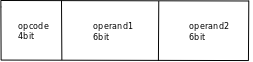
\includegraphics[scale=0.7]{instruction1.png}
\end{center}
Because we have set the lenght of opcode to 4 bits, we could have only 16 = 2²(to the power of 2) But we have 16 opcodes for "real" instructions and 18 "pseudo" instructions without opcode, but they are replaced with composition of actual instructions. For example, instruction "add" opeartes with two registers, saving result of the operation to the left (or first) register:
\begin{verbatim}
movi a 5
movi b 4
add a b
stop
\end{verbatim}
This program will result in:
\begin{verbatim}
program start
PC0 => movi a 7
PC1 => movi b 4
PC2 => add a b
program end
--------------------
registers:
zero: 0
pc: 3
cmp_result: 0
jmp_next: 0
tmp1: 0
tmp2: 0
a: 11
b: 4
c: 0
d: 0
e: 0
f: 0
g: 0
h: 0
\end{verbatim}
Here as first example all registers, that we have are shown, later on only registers, that get some value will be shown. "Program end" - is our "stop" instruction (Mostly known as HALT). So the result is that register a gets the value 11 = 7 + 4. We didn't implement any special output register, cause we can always store (or move to desirable "output"-register) data manually.\\
Both only actual instruction list and all-instruction list can be found in our isa.txt file.\\
Pseudo instructions can be represented by composition of actual instructions. Some of them consist of two instructions, some of them contain up to 5 instructions. For example:
\begin{verbatim}
movi a 7
addi a 5
stop
\end{verbatim}
The original program consist of 3 instructions, but it results in program with 4, because addi is a pseudo instruction replaced with movi and add instructions.
\begin{verbatim}
program start
PC0 => movi a 7
PC1 => movi tmp1 5
PC2 => add a tmp1
program end
--------------------
\end{verbatim}


\end{document}

